% Section 3: A Linear Type System for AI Accountability
% IEEE Computer — "Silent Decisions Are Type Errors"
% Authors: Soares et al., 2026

\section{A Linear Type System for AI Accountability}
\label{sec:type_system}

The accountability gap of Section~\ref{sec:intro} stems from the mismatch
between \emph{sequential} runtime assertions and \emph{concurrent,
high-throughput} AI decision pipelines.  This section introduces the
linear-type framework that closes the gap at the language level.

% ----------------------------------------------------------------
\subsection{Regulatory Obligations as Linear Resources}
\label{sec:linear_resources}

Girard's linear logic~\cite{girard1987linear} treats propositions as
\emph{resources}: each assumption must be used exactly once---no
duplication (\emph{contraction}) and no silent discard
(\emph{weakening}).  This discipline maps directly onto regulatory
accountability obligations.

To support review and explanation under LGPD Art.~20 and EU AI Act
Arts.~14 and~86, BTV models two accountability artifacts as resources.
If an evidence resource could be duplicated,
the same evidence could be recycled across multiple decisions,
undermining causal uniqueness.  If the obligation could be silently
discarded, decisions could escape accountability entirely---the
precise failure mode we call a \emph{silent decision}.  We model the
two obligations as first-class linear types:

\begin{description}
  \item[\texttt{EvidenceToken}]  A linear resource that encapsulates
    the BLAKE3 hash of the decision context (the raw input fed to the
    AI system at inference time).  Construction via
    \texttt{EvidenceToken::new(\&[u8])} binds the token irrevocably
    to a specific context.  The type does not implement \texttt{Clone}
    or \texttt{Copy}, enforcing an ``at most once'' discipline at
    the type-system level.

  \item[\texttt{ComplianceToken}]  A linear resource that encodes the
    applicable regulatory framework: jurisdiction identifier, policy
    version, and contestability deadline in hours.  It is consumed
    by value, binding each regulatory obligation to exactly one
    verdict.
\end{description}

The structural guarantee is narrower than non-repudiation: because an
\texttt{EvidenceToken} cannot be cloned through the public API, one token
cannot be consumed by two verdict constructions.  Tokens can still be
dropped because Rust ownership is affine; what remains mandatory is that
every successful BTV \texttt{Verdict} construction receives both tokens.
We return to the affine-versus-linear discussion in
Section~\ref{sec:binding}.

% ----------------------------------------------------------------
\subsection{The Atomic Binding Operator}
\label{sec:binding}

The central type law of this paper is:
\[
  (E \otimes C) \multimap V
\]
where $V$ denotes \texttt{Verdict}, $E$ denotes \texttt{EvidenceToken},
$C$ denotes \texttt{ComplianceToken}, $\multimap$ is the linear
function type (``linear implication''), and $\otimes$ is the
multiplicative conjunction (``tensor product'') of linear logic.

Reading left-to-right: to produce a $V$, one must jointly
consume exactly one $E$ \emph{and} exactly one $C$.  There is no
partial construction; either both resources are provided and a
verdict is produced, or the program does not type-check
(Figure~\ref{fig:linear_type_law}).

\begin{figure}[t]
\centering
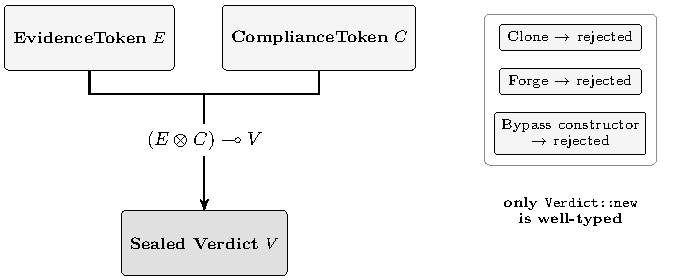
\includegraphics[width=\columnwidth]{figures/fig2_linear_type_law.pdf}
\caption{The core type law $(E \otimes C) \multimap V$: an
  \texttt{EvidenceToken} and a \texttt{ComplianceToken} are jointly
  consumed ($\otimes$) to construct a \texttt{Verdict}. Three bypass
  attempts are rejected by the compiler; \texttt{Verdict::new} is the
  only well-typed path. (The affine-versus-linear discussion in
  Section~\ref{sec:binding} covers the ownership nuance this figure
  omits for clarity.)}
\label{fig:linear_type_law}
\end{figure}

In the implementation, \texttt{Verdict::new} is the concrete
realisation of the $\otimes$-introduction rule
(Axiom~\ref{ax:intro}):

\begin{verbatim}
pub fn new(
    evidence: EvidenceToken,
    compliance: ComplianceToken,
    decision: Decision,
    explanation: String,
) -> Verdict
\end{verbatim}

Both are taken \emph{by value}: after the call, neither token is
accessible to the caller---they have been irreversibly consumed into
\texttt{Verdict}.
The HMAC integrity seal computed inside \texttt{new} binds
\texttt{evidence\_id}, \texttt{decision}, and \texttt{explanation}
into a tamper-evident record, making post-hoc alteration detectable.

\paragraph*{Affine, not strictly linear.}
Precision matters: in substructural-type-theory
terms~\cite{walker2005substructural,pierce2002tapl}, Rust ownership is
\emph{affine} (used zero or one times) rather than strictly
\emph{linear} (exactly once) --- a value can always be silently
dropped. \texttt{\#[must\_use]} on \texttt{EvidenceToken} and
\texttt{ComplianceToken}, plus a crate-level
\texttt{\#![deny(unused\_must\_use)]} (Protection~C,
Table~\ref{tab:protections}), escalates an ignored-return warning to a hard
error, but does not turn Rust into a strictly linear language.
Three escape hatches remain, documented rather than hidden:
\texttt{std::mem::forget(token)} still compiles and leaks the token;
a \texttt{panic!} after construction but before consumption drops it
during unwinding; a process abort loses it with the process. None lets
a \texttt{Verdict} materialize without evidence --- each only discards
evidence, a fail-secure outcome, not a silent decision
(Definition~\ref{def:silent}) --- but they mark the exact boundary of
the "exactly once" guarantee.

This property is stronger than a call-site runtime assertion, which
executes only if the call site is reached and can be omitted from an
untested path; the ownership constraint is enforced by the type
checker and applies to every compilation and every code path.

% ----------------------------------------------------------------
\subsection{Encapsulation as Compile-Time Enforcement Boundary}
\label{sec:encapsulation}

The type law alone is insufficient if an adversary (or an
inattentive developer) can construct a \texttt{Verdict} by other
means---for instance, by writing a struct literal or by directly
assembling the hash value.  Three complementary protections close
the encapsulation perimeter:

% Four columns of identifiers overflowed IEEEtran's single-column measure by
% 72 pt. \footnotesize, terser cells, and @{}-trimmed outer padding fit it.
\begin{table}[t]
\caption{The three protections of the Constitutional Enclosure.  Attack
vectors, left to right: constructing a \texttt{Verdict} by struct literal;
calling \texttt{EvidenceToken::consume()} from outside the crate; and
dropping an \texttt{EvidenceToken} without consuming it.}
\label{tab:protections}
\footnotesize
\begin{tabular}{@{}llll@{}}
\hline
\textbf{ID} & \textbf{Attack vector} & \textbf{Mechanism} & \textbf{Error} \\
\hline
A & Struct literal & Private fields & \texttt{E0451} \\
B & External \texttt{consume()} & \texttt{pub(crate)} & \texttt{E0624} \\
C & Ignored return value & \texttt{\#[must\_use]} & \texttt{unused\_must\_use} \\
\hline
\end{tabular}
\end{table}

Protection~A (Table~\ref{tab:protections}) prevents assembling a
\texttt{Verdict} without the constructor, regardless of the
caller's knowledge of the field types.
Protection~B prevents extracting the inner \texttt{Blake3Hash} for
reuse: the \texttt{pub(crate)} qualifier restricts
\texttt{consume()} to the defining crate, and external calls are
rejected at compile time.
Protection~C turns token discard into a hard error:
\texttt{\#[must\_use]} combined with a crate-level
\texttt{\#![deny(unused\_must\_use)]}.

Together, these three protections form a \emph{closed perimeter}: the
only well-typed path to a \texttt{Verdict} in any external crate is
through \texttt{Verdict::new}, which enforces the $(E \otimes C) \multimap V$
law.

\paragraph*{Scope of the Theorem.}
The Constitutional Enclosure Theorem (Section~\ref{sec:theorem})
holds within the following boundaries:

\begin{itemize}
  \item \textbf{In scope:} All Safe Rust code.  The type checker
    enforces the visibility and ownership rules without exception.
  \item \textbf{Out of scope:} Code using the \texttt{unsafe}
    keyword.  \texttt{unsafe} permits raw pointer manipulation and
    can bypass visibility rules.  Deployments should enforce a
    no-\texttt{unsafe} policy in first-party crates and audit dependencies;
    \texttt{cargo geiger} inventories unsafe usage but does not prove soundness.
  \item \textbf{Out of scope:} Semantic truthfulness of the evidence.
    The theorem guarantees that \emph{some} context was hashed, not
    that the context is the correct or complete input.  Policy-level
    correctness is a separate concern addressed at the application layer.
  \item \textbf{Out of scope:} Policy accuracy.  Whether the
    \texttt{ComplianceToken} accurately reflects the applicable law
    is a legal question, not a type question.
  \item \textbf{Out of scope:} Decisions that bypass the
    \texttt{Verdict} type entirely.  The theorem guarantees that no
    \texttt{Verdict} exists without evidence---it does not guarantee
    that all consequential decisions are routed through
    \texttt{Verdict}.  The pattern \texttt{let \_ =
    EvidenceToken::new(\ldots)} silences the \texttt{\#[must\_use]}
    lint but produces no \texttt{Verdict}, so it is not a silent
    decision under Definition~\ref{def:silent}; routing all decision
    points through BTV is an architectural, not type-level,
    obligation.
\end{itemize}

These boundaries reflect a deliberate separation of concerns: the
public API enforces the \emph{structural} property that a
\texttt{Verdict} cannot be constructed without the required resources;
\emph{substantive} accountability---accurate evidence, correct
policy---belongs to audit, certification, and human review.
